\documentclass[a4paper]{article}


% Because it looks better:
\usepackage{a4wide}
% Take care of input things:
\usepackage[utf8]{inputenc}
\usepackage[T1]{fontenc}
\usepackage{lmodern}
\usepackage{microtype}
% Packages for pictures:
\usepackage{graphicx}
\usepackage{float}
\usepackage{listings}
\lstset{numbers=left, numberstyle=\tiny, numbersep=5pt
,frame=single, captionpos=b}
\lstset{language=Perl}
% Package for urls:
\usepackage{url}
\usepackage{hyperref}
\usepackage{amsmath}
\bibliographystyle{alpha}


% Now let us define a few shortcuts:
% Correct sign for C#:
\newcommand{\CS}{C\nolinebreak\hspace{-.05em}\raisebox{.6ex}{\scriptsize\bf \#\ }}


% --------------------------------------------------------------------------------------------!
%
% NOTE: For better usage of LaTeX with GIT, please write each sentence on an own line, separating paragraphs
%       by the usual double returns. That way GIT can track each sentence on its own instead of always
%       having to track a paragraph as one block.
%
% --------------------------------------------------------------------------------------------!

\begin{document}
\begin{titlepage}
% titelseite
\thispagestyle{empty}



\includegraphics[height=1.8cm]{unilogo_bild}
\hfill

\includegraphics[height=1.8cm]{unilogo_wort}\\[1em]


{\bfseries Universität Ulm} \textbar ~89069 Ulm \textbar ~Germany
\hspace*{38mm}\parbox[t]{38mm}{\bfseries Faculty of \\ Engineering and\\Computer Science\\
\mdseries Institute of Neural\\Information Processing}\\[2cm]

\parbox{140mm}{\bfseries \huge An Exposition of Biological Motion:\\ Weight Effects on Jumping Motion}\\[0.5em]

\parbox{140mm}{Project seminar at Ulm University\\Visual Information Processing \\ WS 2012/2013}\\[3em]

\parbox{140mm}{Andreas Köll, Johannes Bohner \\ Burkhard Hoppenstedt, Tamino Hartmann}\\[4em]



\parbox{140mm}{
{\bfseries\large Abstract}\\
Building on top of the study "Decomposing biological motion: A framework for analysis and synthesis of human gait patterns." [Troje, Journal of Vision, 2002] an algorithm to represent and analyse biological motion was implemented.
Herefor a multitude of test subjects were recorded doing jumping motions (jumping jack / rope skipping) using an active depth camera.
As the to differentiate variable the weight of the subjects was changed for the recording using a weight vest.
The thus collected data was analysed with a statistical method and transformed into a lower dimensional representation.
The resulting classifier was capable of correctly recognizing 75\% of the motions, whether these were with or without the additional weight.
}
\vfill

\parbox{140mm}{\today}



\end{titlepage}

\section{Introduction}

This paper presents \cite{origin} in a different application domain.
We analyzed what the authors did and applied the method on a somewhat different study.
Within the following sections we show the documentation to our work, our conclusions, and how our work compares to the original work.

\section{Biological Motion Decomposition}

This section will briefly highlight interesting and important aspects from the original paper on which our work was based on.
The general goal of the paper was to implement an algorithm capable of interpreting biological motion.
This was done by recording the walking motion of men and women with a motion capturing system on a treadmill and then putting the data through an algorithm to distinguish between the gender based on the biological motion.

As the recorded data was not insignificant in its size, a principle component analysis was used to decrease the data volume.
The original authors found that the first four principal components offered sufficient coverage of the data with a value of 98\%.
Just the poses and their principal components however do not represent movement: they must be animated over time.
This was done by mapping the values to a sinus function modified by its parameters.
The data could then be represented in a single, 229 dimensional vector consisting of three components: the standard poses, the principal components, and the parameters for the sinus function.

The data from all the walkers was then analyzed by a simple linear comparison algorithm.
The trained system managed to correctly classify 90\% correctly in the best case (dependent on the various different variations of the approaches).
This was better than the control group's average.

Finally, the authors inverted the algorithm's processing pipeline to synthesize stylized walkers.
These can be changed interactively, allowing a quick comparison between the two distinct extremes between the genders and any step in between.

\section{Modifications to the Original}

In this section we'll have a closer look on our modifications to the original work.
Our intend was to recreate the original work from ground up with slightly changed parameters.
This meant that we had to do a few things differently, most notably because of the hardware used to record the motion data.

The hardware used restricted us to a more simple motion to capture – basically, it had to be 2D and without any 3D overlaps.
To allow for a higher yield of subjects, we refrained from trying to differentiate gender and instead choose to differentiate between doing the motion with and without weights.
Various experiments with the coverage of the used sensor narrowed the motion we would be using down to 2: jumping jack and rope skipping.

All software used was written by us, based on the algorithms outlined in the original paper.
Basically we created 2 programs: one for recording the motion from the sensor and one for processing the data (although that is more a workflow with many scripts than a complete software).

\subsection{Equipment}

For our recording we used the "Kinect for Windows"\texttrademark \cite{kinect}, connected to a computer running "Microsoft Windows 7"\textregistered \ via USB.
The Kinect is mounted on a tripod to allow correct positioning.
Different weighting conditions for the same subject were achieved with a weight-vest with a weight of 5 kilograms.
For the alternate motion, skipping, we also provided a rope.
We used normal tape to mark positions on the floor so that all recordings were made within a controlled setup.

\subsection{Recording the Data}

The first software allows us to record the skeleton input stream from the Kinect and save it to text files.
We developed the application for recording the input stream from the Kinect in \CS with "Microsoft Visual Studio 2012" utilizing the "Microsoft Kinect Developer Version".
The program is currently available as open source here \cite{csprogram} and can be seen in Fig \ref{fig:programm}.

\begin{figure}
	\centering
	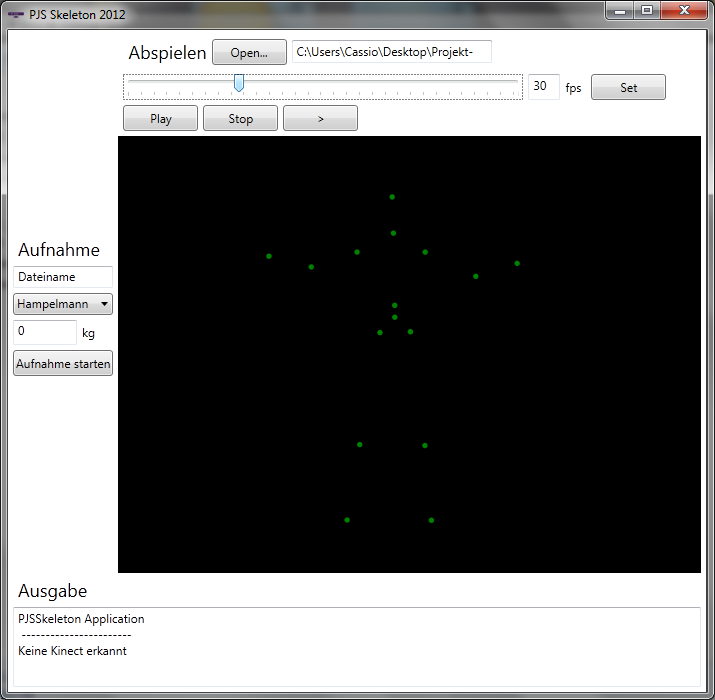
\includegraphics[width=9cm]{programm.jpg}
	\caption{Screenshot of the program used to record the data. The top controls are used to replay a recorded motion, pause and reverse it. Also the frames per second can be adjusted. The center screen shows a point representation of the recorded test subjects joints at the current frame. The controls on the left are used to record a test subject by defining the output filename and a button to start and stop the recording.}
	\label{fig:programm}
\end{figure}


\subsection{Processing the Data}

The other software piece consisted of a multitude of MATLAB \cite{matlabprograms} scripts that were run in sequence on the files to generate our outputs.
Ideally, this should be packaged into a single program too, but we considered the gain to be too small compared to the amount of work required for our project.
Our proposal for this is a node based program where one can manipulate the flow of the data through various external MATLAB scripts; the nodes would be the scripts and the connecting vectors the data moving between them\footnote{An example for the functionality can be found here: \url{http://www.blender.org/development/release-logs/blender-242/blender-composite-nodes/}}.
Such a program could be a future work with a wide array of alternate uses beyond this project.

As the overall workflow of the data from its capture to final results is non-trivial, we have provided a flowchart of the procedure in Fig \ref{fig:workflow}.
The chart should clear up the flow of data in our project from the recording to the various intermediate steps to our final results.

\begin{figure}
	\centering
	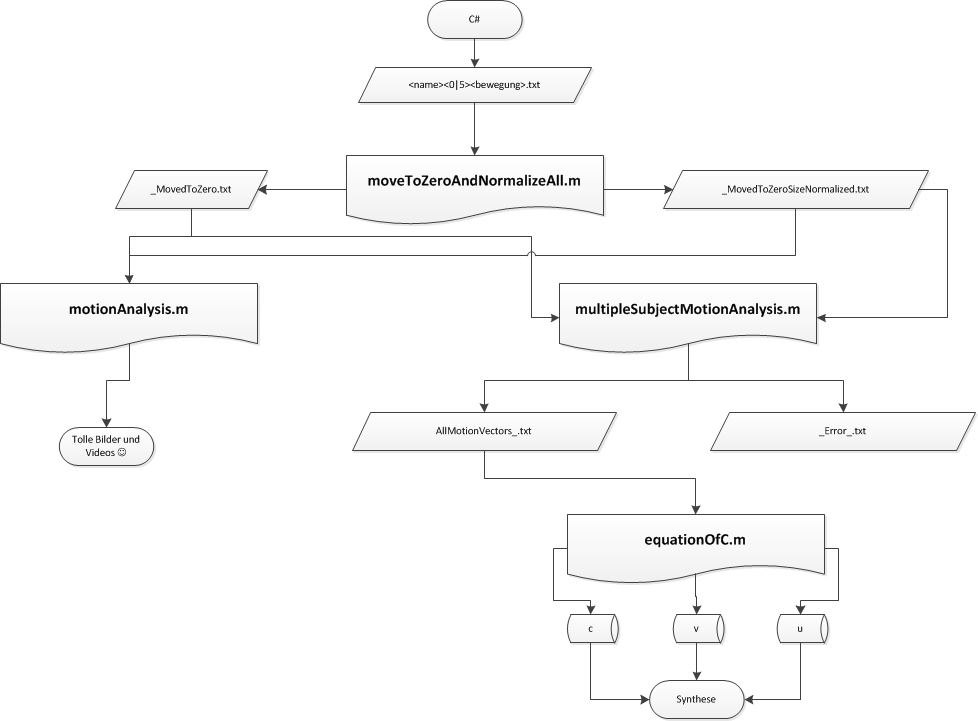
\includegraphics[width=16cm]{matlabaufbau.png}
	% Bei der caption kann ich kein \CS verwenden, also habe ich C-sharp geschrieben.
	\caption{Overview of the workflow of the data. The data enters the workflow at the C-sharp node at the top, written into a text file labeled according to the parameters of the recording. Emboldened nodes mark the MATLAB scripts that processed the raw data into more refined data. Note that the output data was always saved as text between steps too. This allowed a very flexible workflow. For creating the pictures and videos, motionAnalysis.m was used. The other branch of nodes is used to synthesize data.}
	\label{fig:workflow}
\end{figure}

\subsection{Composition of the Recording}

Figure \ref{fig:schematic} shows the schematics of the arrangement of the Kinect for the recordings.
The way the Kinect records skeletons proved to be a strong limiting factor in selecting which motions to record as the depth-perception is comparatively poor.
The fixed nature of the experiment also limited the motion to one that could be done within a small area, which excludes for example any form of walking or running.

\begin{figure}
	\centering
	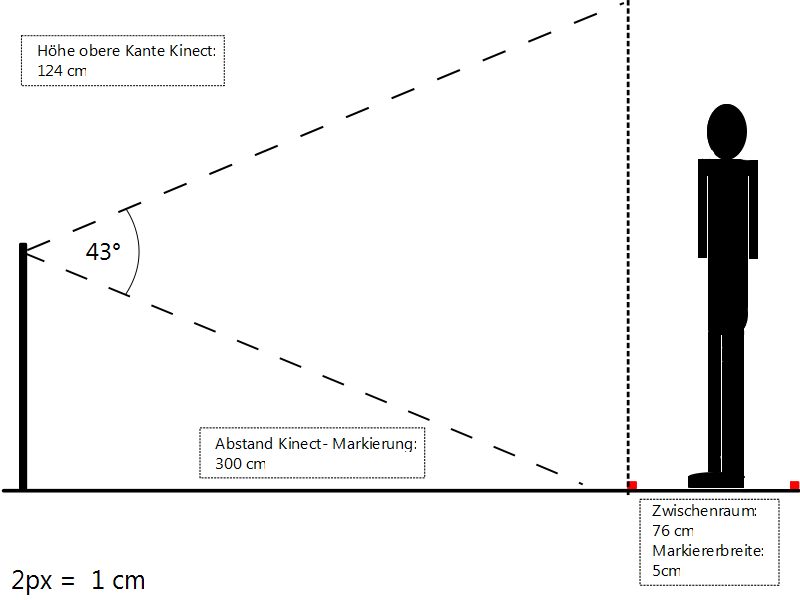
\includegraphics[width=10cm]{Aufbauohnelizenz.png}
	\caption{Schematics of the arrangement for the recording of our source data. On top of the pole to the left the Kinect is mounted. The dashed lines show the field of view. The mannequin shows where the subjects were asked to perform so that the sensor could record under ideal conditions.}
	\label{fig:schematic}
\end{figure}

\subsection{Recording Subjects}

Once everything was in place and we were relatively comfortable with our software and the process of recording, we asked random acquaintances to be subjects in our project.
Each subject had to do either or both of the motions with and without the weights on them.
We thus recorded 19 data sets of the jumping jack and 16 data sets of the rope skipping.
Each data set consists of one recording with the weight and one without.
The order in which the subjects either started or finished with the weight was equally distributed among the group to minimize effects of fatigue.

As the Kinect senses the 3D spatial information via infrared, we initially had trouble when test subjects wore dark clothing.
This was due to the dark clothing absorbing the infrared, thus becoming invisible to the Kinect.
To solve this problem, we had all subjects that wore dark clothing wear a blue overall over their clothes to assure a steady recording.

For the actual recording, we first explained the procedure to our subjects.
This was done to ensure that all captured movement data would generally have the same form of the motion.
We then had the subjects start with the motion and then pressed record.
For the recording of jumping jacks, our software automatically recognized the start position and counted 10 cycles of jumping jacks.
These 10 cycles were then saved in a text file consisting of the 3D vectors of the 16 skeleton points over the frames in time.

An example of the recording can be seen here: \url{http://youtu.be/CJLkOyAGtjk}. The Kinect stands to the right of the camera, at the same relative distance.

\section{Creating Motionvectors to Represent Motion Data}

Having saved all of the skeleton data received from the Kinect into text files, the representation of the jumping motion of every subject is a huge matrix.
Each row of this matrix represents one single posture of the subject's body consisting of 48 values.
Each of the 16 joints is represented by three floating-point numbers specifying the three-dimensional position of the joint.
The postures can also be seen as points in the 48 dimensional space.

This data is highly redundant.
For example, jumping jack and jump rope are symmetrical motions.
The right arm moves the same way as the left arm does, except that it is mirrored.
The same goes for the legs.

Therefore we hoped that the dimensionality of the postures could be drastically reduced without losing much of the information within the data using principal component analysis (henceforth referred to as PCA).
Basically, what the PCA does is to rotate and move the 48 dimensional Cartesian coordinate system in which every possible three-dimensional 16-joint-skeleton posture can be represented as one point, so that for all n $\in \left\{1, ..., 48\right\}$ the first n axes account for as much as possible of the variance of the postures of one subject's jumping motion.
The vectors that represent the axes of the transformed coordinate system are called the principal components.
The origin of this coordinate system is the average of all postures, which we are going to refer to as average posture $p_{0}$.
The principal components are the eigenvectors of the covariance matrix of the skeleton data set.
Like in \cite{origin} we are going to refer to these eigenvectors as "eigenpostures" to distinguish them from the eigenvectors of another PCA we are going to use later.

\subsection{Sinusoidal--Approximation of Coefficients}
A graphical representation of an \emph{eigenposture} for a jumping jack motion can be seen at the top of figure \ref{fig:approx}.
Here the blue curve represents the first coefficient of the \emph{eigenposture} and the green curve the second coefficient.
Apparently this graph looks similar to a sinusoidal graph.
The reason for this characteristic is that our jumping motions are cyclic motions.
Therefore the coefficients of our \emph{eigenpostures} can be approximated using sinusoidal functions.
This is done similar to the approach of \cite{origin}.
Hereby a sine function is used to describe each of the coefficients of the \emph{eigenposture}.
The approximation is done using MATLAB's integrated \emph{fit} function.
The fitted graph of the example mentioned above can be seen at the bottom of figure \ref{fig:approx}.

\begin{figure}
		\centering
		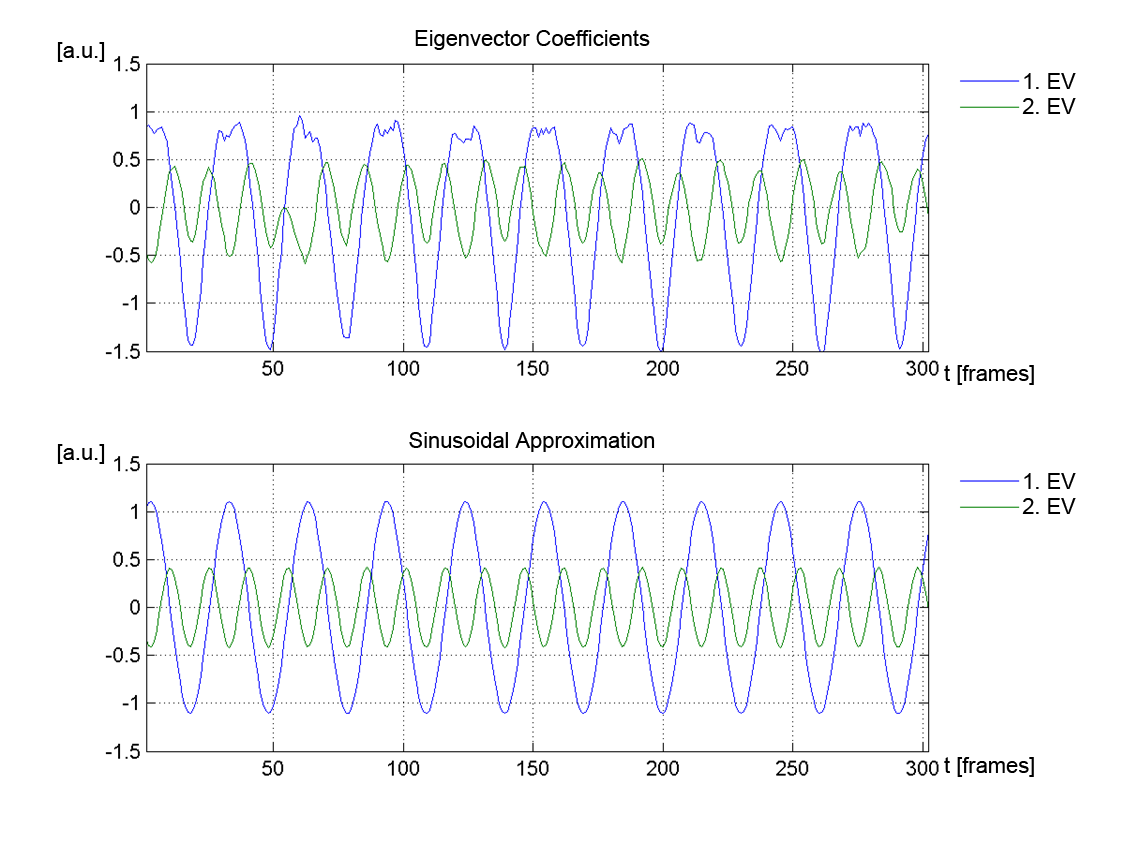
\includegraphics[width=\textwidth]{1sinHamp.png}
		\caption{Original recorded dataset (top) and sinusoidal approximation of coefficients using one sine function (bottom).
		Comparing the two graphs we can see that the first wave's top curve is approximated inaccurately but also the second wave's irregularity cannot be fitted well.
		Which both results in a fit that is not optimal.}
		\label{fig:approx}
\end{figure}

MATLAB's \emph{fit} function also outputs the goodness of the fit in form of the square of the correlation (\emph{rsquare}).
Here values close to zero mean a bad fit and values close to one a good fit.
A value of one would be an exact fit with no information lost.
The goodness of the fit shown in figure \ref{fig:approx} is 0.90225 for the first and 0.80946 for the second coefficient.
This is a rather good result considering that we used a motion of ten full cycles as input and every difference in each of the cycles impairs the approximation.
Also the approximation goodness of this example is close the the average goodness of all our jumping jack \emph{eigenpostures}.
This also counts for the following examples.

Also when looking back at our jumping jack example in figure \ref{fig:approx} we can see that especially the first coefficient is rather badly approximated on the top of the wave.
We tried therefore an additional approach to get even better results. That is to use two overlapping sine functions for a better representation of each coefficient.
The result of this approach can be seen in figure \ref{fig:approx2}.
Here the \emph{rsquare} values are 0.98515 for the first and 0.9366 for the second coefficient and thus represents a better model of our jumping jack motion.

\begin{figure}
		\centering
		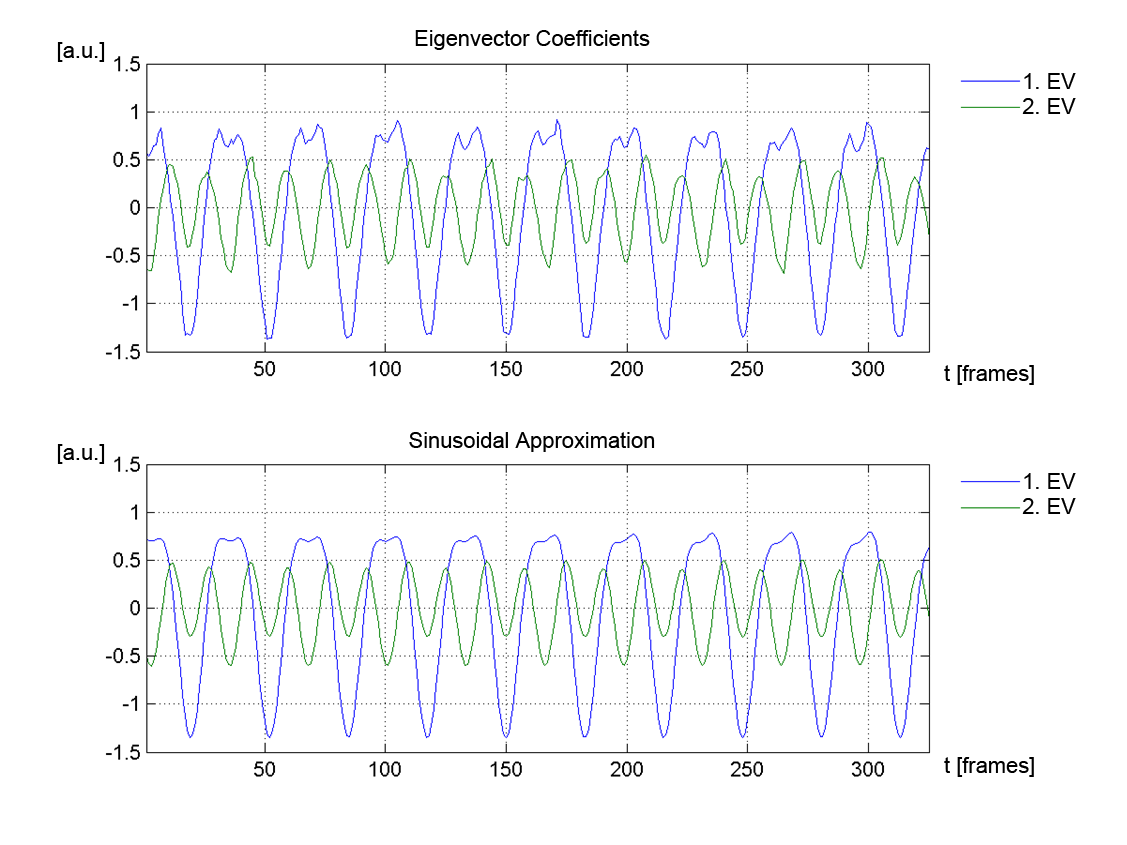
\includegraphics[width=\textwidth]{2sinHamp.png}
		\caption{Original recorded dataset (top) and sinusoidal approximation of coefficients using two overlapping sine functions (bottom).
		The approximation of the first wave's top curve is much closer to the original data compared to the usage of only one sine function.
		But also the second wave's approximation matches the original data very closely.
		Therefore this is a better model for the jumping jack motion.}
		\label{fig:approx2}
\end{figure}

The rope skipping motion, as seen in figure \ref{fig:approx3}, however does not have this characteristic so here only one sine function was used for our further work.
The \emph{rsquare} values here are 0.98886 and 0.84932 for the two coefficients.

\begin{figure}
		\centering
		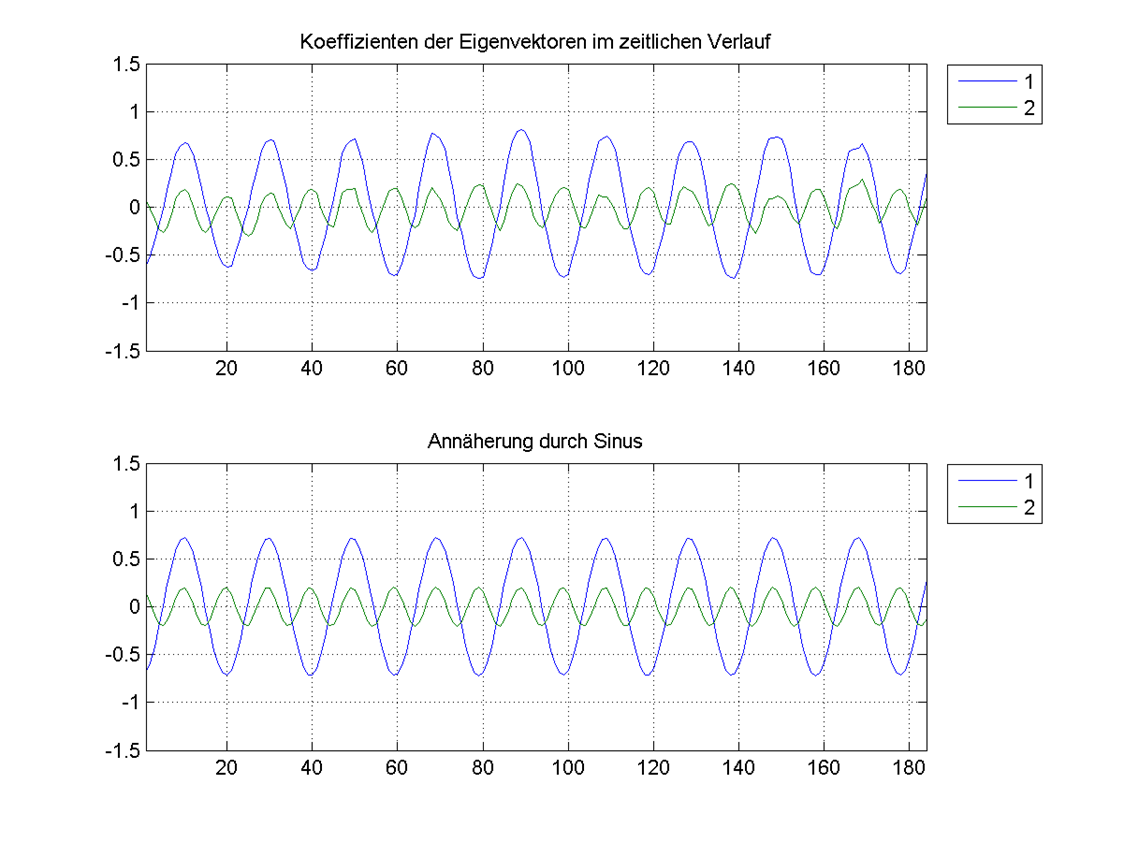
\includegraphics[width=\textwidth]{1sinSeil.png}
		\caption{Original dataset of a rope skipping motion (top) and its sinusoidal approximation (bottom).
		In contrary to the jumping jack approximation this works very well using only one sine function.}
		\label{fig:approx3}
\end{figure}

\subsection{Normalization}
While jumping there are unwanted side-effects. People can't continuously jump just up and down, but also back- and sidewards. This fact effects our first two eigenvectors. They loose importance in representing the whole movement. So we idealize the movement by removing all changes to the z-axis. The result can be seen in figure \ref{fig:sammel}.

% Was ist mit normalisieren der Hüfte auf x? 

\begin{figure}
	\centering
	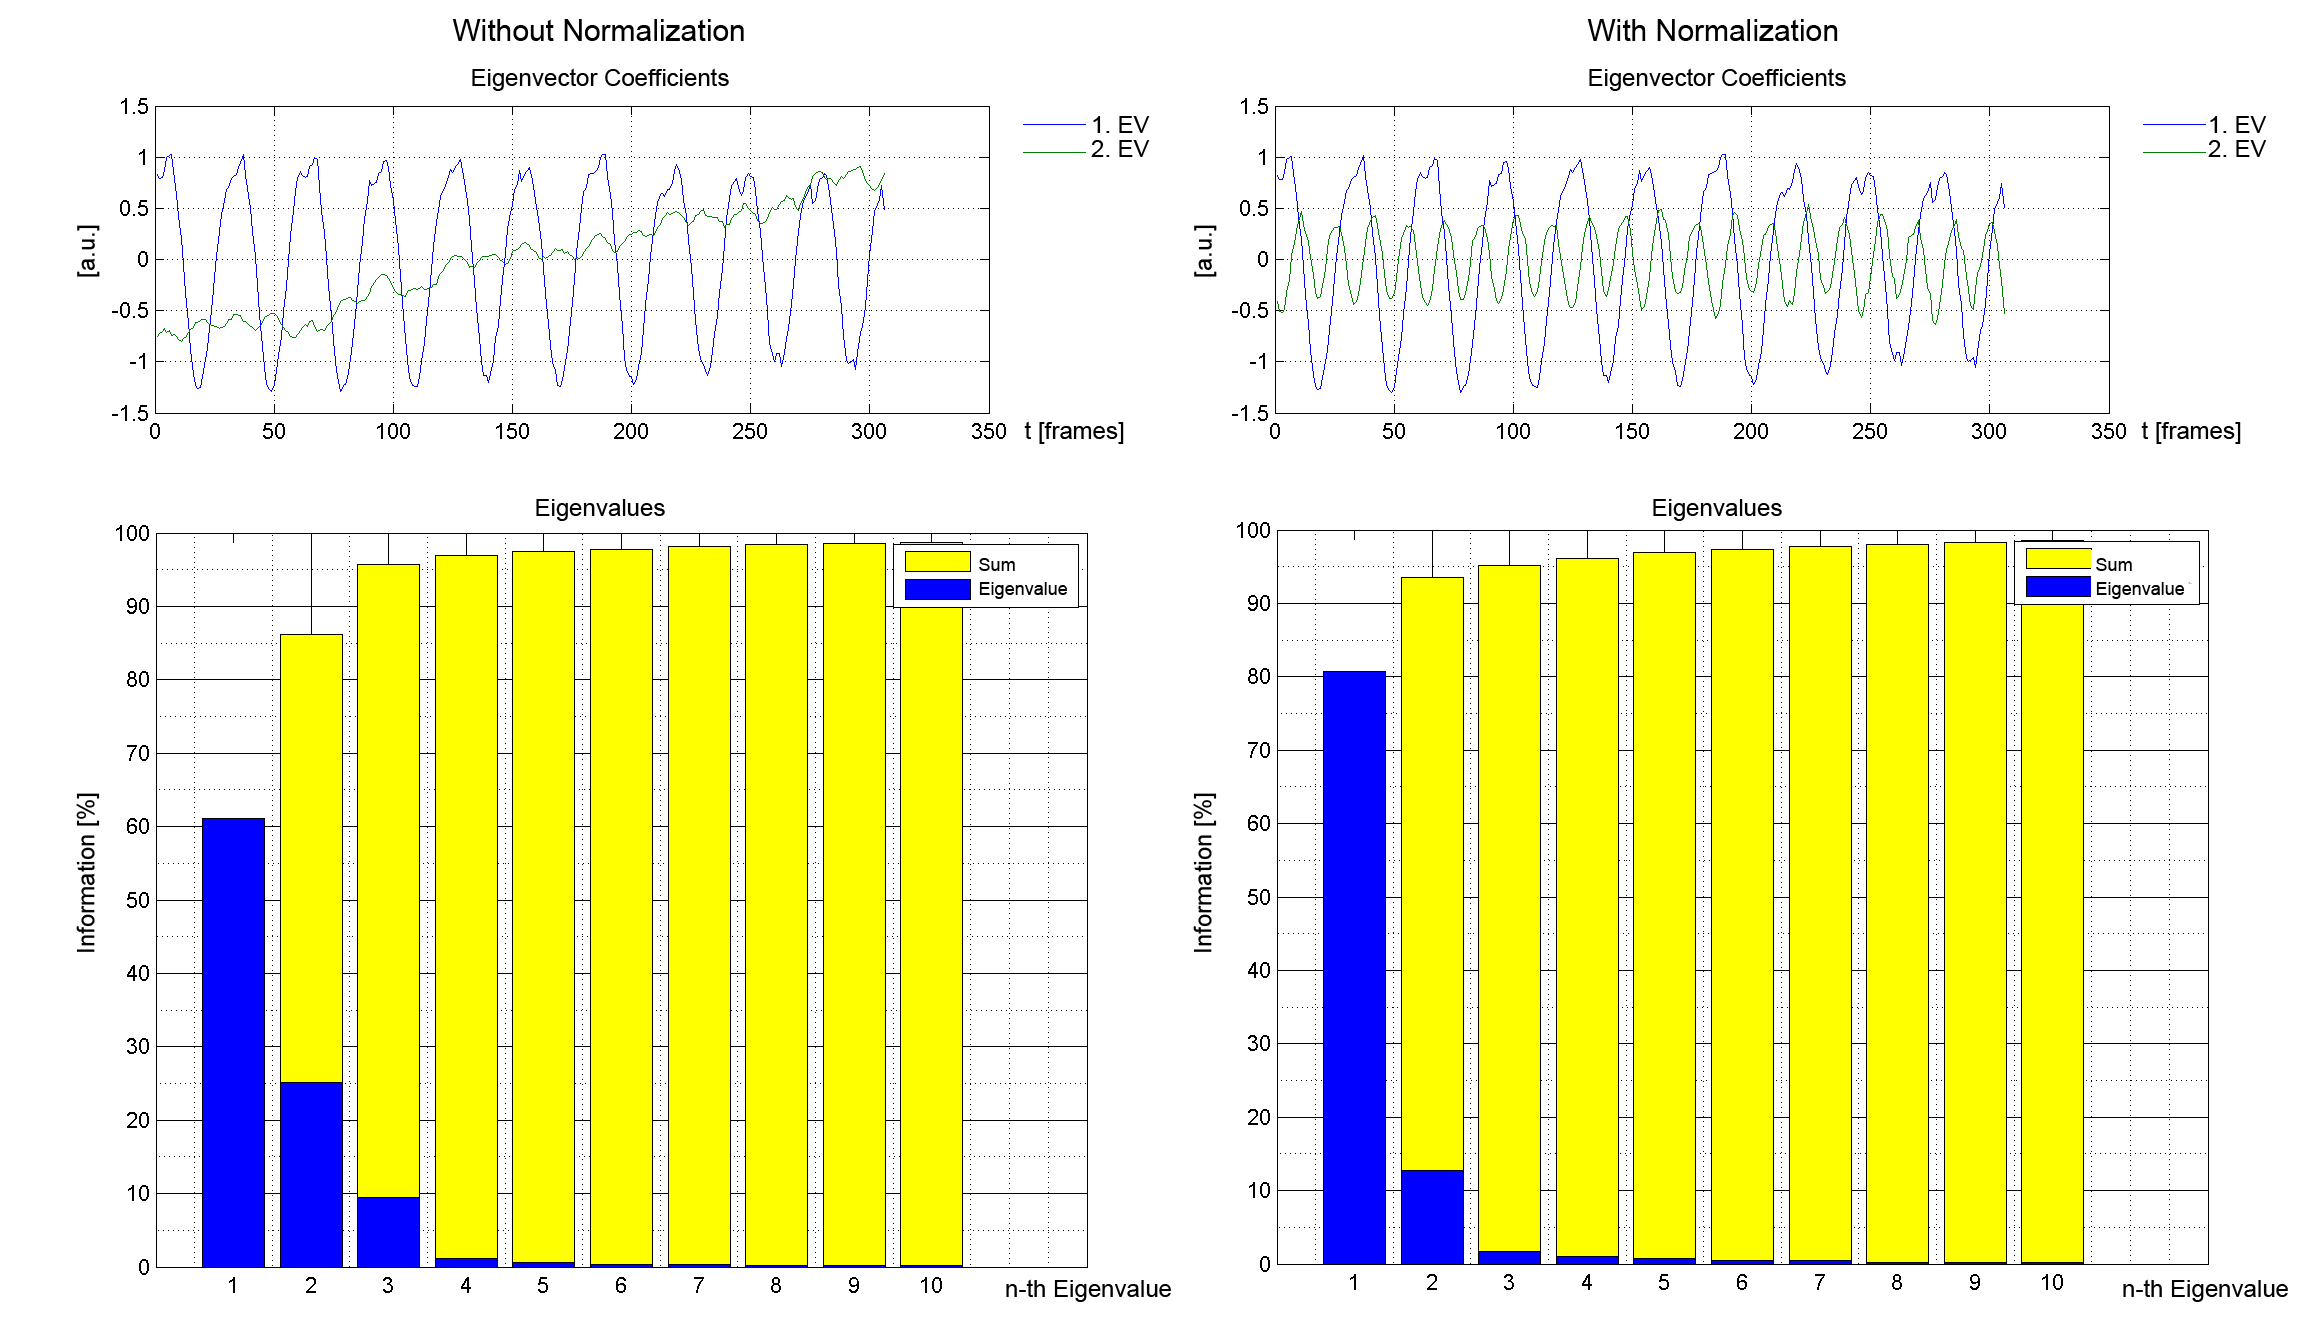
\includegraphics[width=15cm]{sammel.png}
	\caption{Normalization effect on coefficients. The top left graph shows the sinusoidal approximation a recorded motion without any normalization. Here the second eigenvector's coefficients show a linear noncyclic behavior over the length of the recording.
	Also more eigenvalues of the PCA result are needed to cover most variance.
	Using normalization the negative effects can be eliminated and the second eigenvector's wave behaves cyclic as we would have expected.}
	\label{fig:sammel}
\end{figure}

\subsection{Comparison of original and after-processing-motions}

% TODO Animationen vergleichen / in pdf einbinden?

\subsection{Creation of Motion Vectors}
To create a motion vector, which is to describe the full motion cycle using our sinusoidal approximation, we need the average posture created earlier and the first two \emph{eigenpostures} including the sinusoidal approximation of their coefficients.
However due to the normalization mentioned earlier we don't need all three positional values of our skeleton points, but can ignore X and Z values for the hip.
Therefore we have three positional values X,Y,Z for 15 skeleton points and only one additional for the hip resulting in 48 values for each posture.
To describe the sinusoidal approximation we use different setups for our four options.

When using one sine wave for each \emph{eigenposture} and the jumping jack motion, it is sufficient to track the wave's amplitude for each posture and one frequency since the second wave's frequency is exactly twice the first one's for all test subjects.
Also, as the waves are in phase for all test subjects we did not have to track the phases.
This results in motion vector of 141 dimensions to describe the jumping jack motion.

When using two sine waves for each of the \emph{eigenpostures} and the jumping jack motion, we need to track the four wave's amplitudes the frequency and three phases relative to the first wave's phase.
This results in a 146 dimensional motion vector.

When using two overlapping sine waves for the first and one sine wave for the second \emph{eigenposture} on the jumping jack motion, we need to track the three wave's amplitudes the frequency and two phases relative to the first waves's phase.
This results in a 144 dimensional motion vector.

For our rope skipping motion we need the two amplitudes but also two frequencies as there is no recognisable pattern in the waves.
It appears to be a multiple of the first frequency for some test subjects but not always the double.
Also one phase is needed for the second wave relative to the first one.
This results in a 143 dimensional motion vector for the rope skipping motion.

% TODO Testpersonen, wohin? Von Tamino: ist doch oben...? Oder wird hier was anderes gemeint? % die Folie "Testpersonen" mit den geeigneten personen pro option -> grund für die 2+1 geschichte

\section{Results}

For now each jumping motion is represented by a 141/143/144/146-dimensional motionvector.
Earlier we used PCA to reduce the dimensionality of all 48-dimensional representations of skeleton postures of one single jumping motion.
Now we are going to do the same with all the 141/143/144/146-dimensional representations of the complete jumping motions.

\subsection{Using Standard Deviations to Normalize Motionvectors}

However this time the dissimilarity of the data in the motionvectors might affect how well the PCA will work.
The first PCA's input were 48-dimensional postures where each of the 48 entries was a distance describing one dimension of the three-dimensional position of one joint.
All of the entries in each posture were comparable.
The entries in the motionvector, however, describe positions, frequencies, amplitudes and phases, thus the values of one motionvector has various magnitudes.
Therefore we created a 141/143/144/146-dimensional standard deviation vector u containing the standard deviations of each motionvector-entry of the complete set of motionvectors.
Each entry of each motionvector was then divided by the corresponding entry of u prior to running the PCA.
The vector u was saved to a file for later use.

\subsection{Running a PCA on the Motionvectors}

The result of this second PCA is another set of eigenvectors, which we are going to refer to as the eigenjumpers, comparable to the eigenwalkers of \cite{origin}, and for each jumping motion a set of coefficients (also called weights or scores).
Given the eigenjumpers and the average motionvector one can reconstruct any motionvector by using the coefficients that belong to the motionvector. Exactly as with the first PCA this is achieved by adding up the average motionvector to the sum of the products of each eigenjumper and its corresponding coefficient.
For this reason the coefficients that belong to one subject's data are another representation of this subject's jumping motion.
The matrix K contains these coefficients. Each row of K consists of one subject's jumping motion. In the following we will use $k_{i}$ as a name for the i-th row of K, being the coefficients of the i-th jumping motion.
Due to the PCA the entries in the beginning of each row contribute the most to the representation of the jumping motion, whereas the entries in the end of the row contain little information and might be omitted.
As we will see later the choice of how many of the coefficients we are going to use for classification is an important one, because too few coeffiecients might not be an adequate representation of the motion, while too many coefficients will describe each motion too specifically and therefore might be difficult to classify.

\subsection{Creating the Classifier c}

To create the classifier, a resultvector r was defined containing one entry for each of the recorded motions. The corresponding entry was 1 if the subject performing the motion was wearing the weight-vest, if this wasn't the case the entry was -1. The classifier c was then created by solving the linear equation system
\begin{align}
	K \cdot c=r \label{eq:cEquation}
\end{align} 
(Note: This is different from the equation in \cite{origin}, because there the coefficients of one walking motion were contained in one column of K, rather than in one row as K is defined here.)

The number of coefficients was more than 140, which is far more than the number of recorded jumping motions. This means, that the linear equation system \ref{eq:cEquation} cannot be solved uniquely. There is an infinity number of possible solutions of c. Since the most important entries of c would be the ones in the beginning (because they will correspond to the more important coefficients in K), a solution for c was chosen, in which as much as possible of the entries in the end were set 0. This means only the entries at the beginning of c contained valuable information.

\subsection{Classifying Jumping Motions}

Any of the recorded jumpin motions can be classified by building the dot product of the corresponding coefficients and the classifier c.
Due to the defintion of c, the result of this dot product is either 1 or -1, indicating whether the jumping motion was performed with or without the weight-vest.
As mentioned earlier, most of the information about a motion is contained in the entries at the beginning.
It is now examined how well the classifier works if it is not used completely, but rather only the first n entries of c and $k_{i}$ were used to determine whether the weight-vest influenced the i-th jumping motion or not.
Instead of the dot product, the term
\begin{align}
	D=\sum\limits_{j=1}^n c_{j} k_{i,j} \label{eq:dotproduct}
\end{align} 
was applied. If the result was positive, it was classified as weight-burdened motion, otherwise, it was classified as unburdened motion.
Naturally, for small n the error rate was quite high getting smaller for increasing n.
One can easily comprehend, that there are no more misclassifications when n reaches the number of jumping motions, because this is the number of nonzero entries in c, all of the following entries are 0, anyways.
For an n equal to or higher than the number of recorded motions, the result of the equation \ref{eq:dotproduct} is therefore always 1 or -1, because the entries after the n-th entry don't contribute anything to the sum.
For an n smaller than the number of motions, the result of the sum might be different than 1 or -1, but the sign might still be sufficient to classify the motion correctly.

The blue curves in figure \ref{fig:classification} show the percentage number of misclassifications depending on n, the number of used entries of c and $k_{i}$. As you can see, there usually is an n smaller than the number of motions for which is already high enough to classify all motions correctly.

\begin{figure}
		\centering
		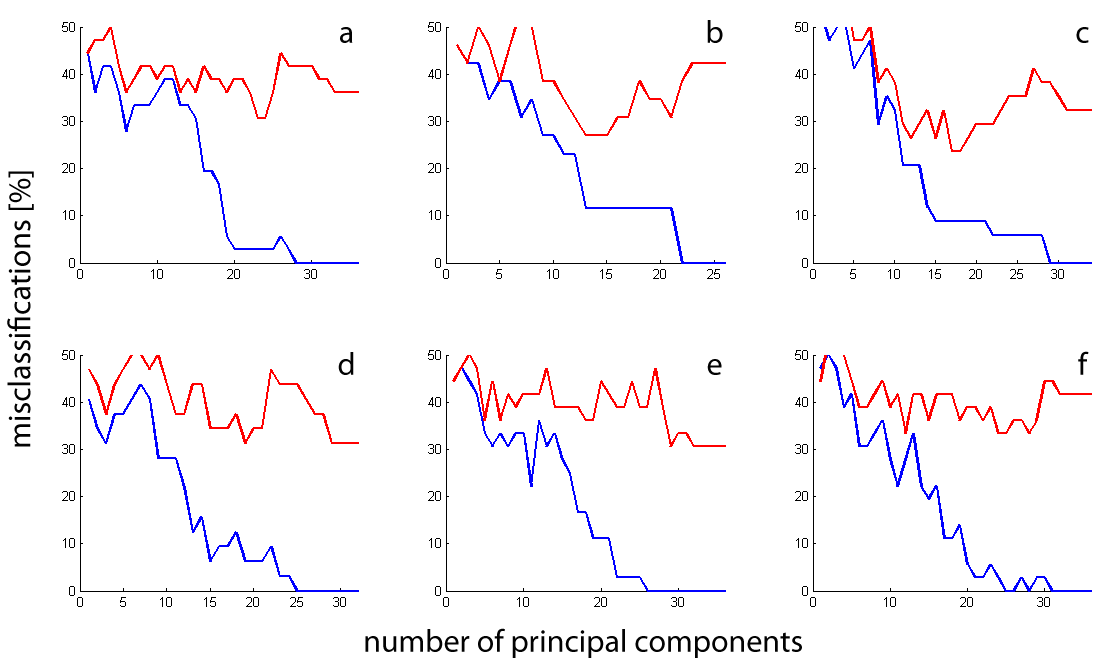
\includegraphics[width=\textwidth]{klassifikation.png}
		\caption{Classification errors depending on the number of used principal components.
		The blue curve shows the number of misclassifications using the universal classifier that was trained with all the motionvectors, the red curve depicts the misclassified motionvectors using the leave-one-out-strategy.
		The following types of motionvectors were classified here:
		a: jumping jack using one sine wave for both eigenpostures
		b: jumping jack using the sum of two sine waves for both eigenpostures
		c: jumping jack using two sine waves for the first eigenposture and one for the second
		d: jumping jack, only average posture (structural information)
		e: jumping jack, all entries except average posture (dynamic information), one sine wave for both eigenpostures
		f: jumping jack, only first and second eigenposture (dynamic information)
		g: rope skipping
		h: rope skipping, only average posture (structural information)
		i: rope skipping, only first and second eigenposture (dynamic information)}
		\label{fig:classification}
\end{figure}

\subsection{The Leave-One-Out-Strategy}

For now we only had one classifier c trained by all the recorded motions.
For a sufficiently large number of used principal components this classifier can classify all of the motions correctly.
A far more interesting question is, how well the classifier will work for a new jumping motion that wasn't used to train it.
For this reason \cite{origin} used a leave-one-out-strategy, taking one out of the set of recorded walkers and computing the classifier c for the remaining walkers.
In our work we took out one subject's two motionvectors (one of them weight-burdened, the other one burdenless) and classified both of them using the classifier trained by the other motionvectors.
The classification was determined by projecting the motionvectors that were to be classified onto the eigenjumpers of the other motionvectors, applying the equation \ref{eq:dotproduct} to both of them.
This was repeated for all subject's motionvectors, until all of them have been taken out and were classified.
The number of misclassifications is shown as the red curves in figure \ref{fig:classification} as a function of the number of used principal components.

Figure \ref{fig:classification} (a) shows the misclassifications using the 141-dimensional motionvector jumping jack representation that uses only one sine wave to represent the coefficients of each eigenposture.
At the minimum about 30\% of the recorded motions were misclassified using about 24 principal components.
This was improved slightly to 27\% misclassifications in figure \ref{fig:classification} (b) using the 146-dimensional jumping jack motionvectors that utilized the sum of two sine waves to represent the coefficients of each eigenposture.
Even though the 144-dimensional jumping jack representation that uses two cumulative sine waves for the first eigenposture and only one sine wave for the second eigenposture is a worse representation than the 146-dimensional one with two sine waves for each eigenposture, the former one has a better misclassification rate of less than 25\%, because more of the recorded jumping jack motions were applicable to this 144-dimensional representation.
This is shown in figure \ref{fig:classification} (c).
The minimum of about 24\% is achievied by using about 17 principal components.

Rope skipping in figure \ref{fig:classification} (g) had a minimum error rate of less than one third using 19 principal components.

\subsection{Classification Using Only Parts of the Motionvectors}

The curves in figure \ref{fig:classification} (d), (e), (f), (h) and (i) show the error rate of jumping motions using only parts of the motionvector. (d), (e) and (f) show the classification of jumping jack, (h) and (i) rope skipping.
In (d) and (h) the first 46 entries, the average postures, of the motionvector were used: that means the structural data of the motionvector.
In \cite{origin} it turned out, that this kind of data wasn't essential for gender-classification.
We experienced the same with the rope skipping motion: weight-burden classification didn't work well.
For the jumping jack, however, the minimum classification error using only the average posture was clearly smaller than 30\%.
A possible explanation for this is that the average posture contains information about a subject's weight-burden, because the weight-vest would push a subject down to the floor, influencing its posture.

(e) shows the jumping jack (one sine wave for both eigenpostures) classification using all the motionvector's entries except the average posture being the dynamic information of the motionvector.
The curves show, that this doesn't work well for classification.

In \cite{origin} the best result for classification was achieved using the first three eigenpostures.
In (f) and (i) everything but the first two eigenpostures were used for classification resulting in a minimum error of about 22\% each.
This is so far the best result.

We see that for rope skipping using only the two eigenpostures seems to work clearly better than using the complete motionvector. For jumping jack the difference of minimum misclassifications between (i) and (c) is really small. Further studies would be necessary to determine which method works better.

\section{Synthesizing of Jumping Motions}

Given a motionvector, the original motion can be restored by computing the coefficients and then building the weighted sum of the average posture and the eigenpostures using the coefficients.
Jumping patterns can therefore be synthesized, by creating new motionvectors.

\subsection{Difference Vector Synthesizing}

A simple, intuitive way to do so is to calculate the average motionvector of weight-burdened motionvectors and the one of the unburdened motions (using motionvectors that weren't divided by the standard deviations first).
These average motionvectors can be seen as two points in the 141/143/144/146-dimensional space.
It would be interesting to have a closer look to the motionvectors lying on the straight line defined by these two points.
The points that lie beyond any of the two motionvectors would be exaggerations, either showing a really heavy burdened jumping motion or a very light unburdened motion.
These points were calculated by building the difference between the two average points (the vector pointing from one of the points to the other) multiplying the result by a freely choosable weight $\alpha \in R$ and adding this to the average of all the motionvectors.
The most eye-catching feature of the resulting animation was that a highly exaggerated burdenless jumper was jumping much faster than an exaggerated weight-burdened jumper.
Sadly the difference in speed was so high, that other features almost weren't visible in the animation.
Therefore we changed the difference vector dividing the entry that contained the frequency by 10.
In the animation, the exaggerated unburdened jumper was still faster than its burdened equivalent, but the difference in speed was growing slower with an increasing level of exaggeration.
Other features were therefore observable in the animations.
The unburdened jumper jumped higher raising its hands far above his head.
Its average posture also was clearly higher than the burdened jumper whose motions appeared to be small in the vertical direction.

\subsection{Synthesizing Using the Classifier}

For computing the TODO: TEXT?
Before the classifier c was computed, the motionvectors were divided by the standard deviations. These were saved as the vector u to a file.

\section{Visualization}

This section is independent from the rest of the paper as the analytical methods don't matter.
Our intent is to show the captured points of the skeleton in an representative 3D Model.

\subsection{Absolute vs. Relative Values}

As seen in the description of storing points in a ".txt" file the Kinect uses absolute values to represent the skeleton  - which is absolutely useful, because otherwise it couldn't detect different lengths in body parts.
Instead it would have to map the measured values onto a defined body model.
This procedure would cause inaccuracy.
While animating a defined model in the opposite you can't just easily scale single body parts to adjust the proportions.
This problem requires a solution in a format invariant to scaling.

\subsection{The .bvh File}

The software used for testing the following part is SmithMicro's Poser 9.\footnote{http://www.software3d.de/figurendesign/smithmicro-poser-9.html}
A .bvh file is made up of two parts: The body structure and the frames.
The body structure defines the relationship between each body part.
As one might see in Listing 1 this structure is build hierarchical.
Each joint is represented by a name and the connection to its successors.
Changing the value in a joint affects all the successors. 
The standard pose (all angles in between 0) is the so called T-Pose.
You can see the model standing with parallel feet looking straight forward and the arms are bend 90 degrees relative to the body.

\begin{lstlisting}[caption=.bvh Connected Structure. TODO: MORE TEXT!]{Name}
JOINT lCollar
{
		OFFSET	1.858774 10.237258 -1.915852
		CHANNELS 3 Zrotation Yrotation Xrotation
		JOINT lShldr
		{
			OFFSET	6.103279 0.000102 -0.038601
			CHANNELS 3 Zrotation Yrotation Xrotation
			JOINT lForeArm
\end{lstlisting}

Responsible for the change over time is the second part of the file.
There we define the joint-angles.
Really useful for this aspect of the project was the similarity between the recorded ".txt" file and the second part of the ".bvh".
Therefore we could calculate the absolute positions in a row from the .txt-file to angles and replace the current lines in the .bvh by the ones generated by a MATLAB script which will be shown in the following section.

\begin{lstlisting}[caption=Motionpart of .bvh. TODO: MORE TEXT!]{Name}
MOTION
Frames:     160
Frame Time: 1                
0 50.946 0 0 0 0 0 0 0 0 0 0 0 0 0 0 -30.66 0 0 -30.295 0 0 10.811 ...
0 51.229 0 0 0 0 0 0 0 0 0 0 0 0 0 0 -29.93 0 0 -30.695 0 0 9.6152 ...
\end{lstlisting}

\subsection{Calculating the angles}

After finding the corresponding entries in the ".txt" and ".bvh" file now is the time to convert values.
Using MATLAB as an intermediary between the two formats we take the advantage of the easy handling of .txt to matrices.

The problem is now solved by the vector based equation: $\vec a \cdot \vec b = \left|\vec a \right| \left|\vec b \right| \cos \phi$.

\begin{lstlisting}[caption=Calculating the angle. TODO: MORE TEXT!]{Name}
D = dlmread('nameSeilhuepfen0.txt');
[...]

# right upper arm entry #25 (vector 24x data is already here)
m46 = (D(ind,17)-D(ind,11))/(D(ind,16)-D(ind,10));

# Vector calculations. Enumeration is from point number
#       from Kinect model
vector46y = D(ind,17)-D(ind,11);
vevtor46x = D(ind,16)-D(ind,10);
dotproduct=vector24y*vector46y+vector24x*vector46x;
lengthOne=sqrt(vector24y^2 + vector24x^2);
lengthTwo=sqrt(vector46y^2 + vector46x^2); 
wUpperArmRight = radtodeg(acos(dotproduct/(lengthOne*lengthTwo)));
\end{lstlisting}

\begin{figure}
	\centering
	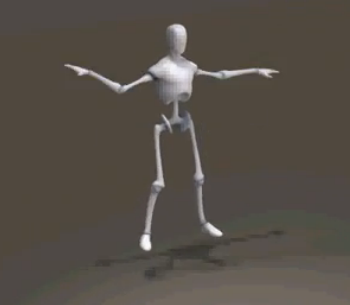
\includegraphics[width=8cm]{3dRender.PNG}
	\caption{Result of rendering in Poser. This is a still from the jumping jack motion using our data transformed into the correct format.}
	\label{fig:3drender}
\end{figure}

\newpage
\bibliography{doc}

\end{document}
